\chapter{Introduction}
\label{ch:intro}
\par The Sun is the most important celestial body to life on Earth. For the last five billion years, it has provided the light by which humans observe the world around them and the heat to save the planet from the frigid temperatures of interplanetary space. Because of its proximity, the Sun provides astronomers an exclusive and unique look into how stars behave. By observing and understanding the Sun, one can make conclusions about other types of stars in our galaxy and the universe.
%
\par Perhaps no other consistent celestial event has attracted as much attention as the solar eclipse. Solar eclipses have been observed and recorded for thousands of years, with some reports dating back to the fourteenth century BC \citep{golub_solar_2010}. The recordings of ancient eclipses have been heavily studied. Chinese rock drawings dating back to the Han dynasty (approximately 1900 years ago) appear to show the moon completely obscuring the Sun. Additionally, some have even suggested the Aubrey holes that surround the Stonehenge site were used to track and predict both solar and lunar eclipses \citep{golub_solar_2010}. Though some claims of ancient eclipse studies are controversial, it suffices to say that humans have long sought to study and explain the behavior of the nearest star to Earth.
%
\begin{figure}[htbp]
	\centering
	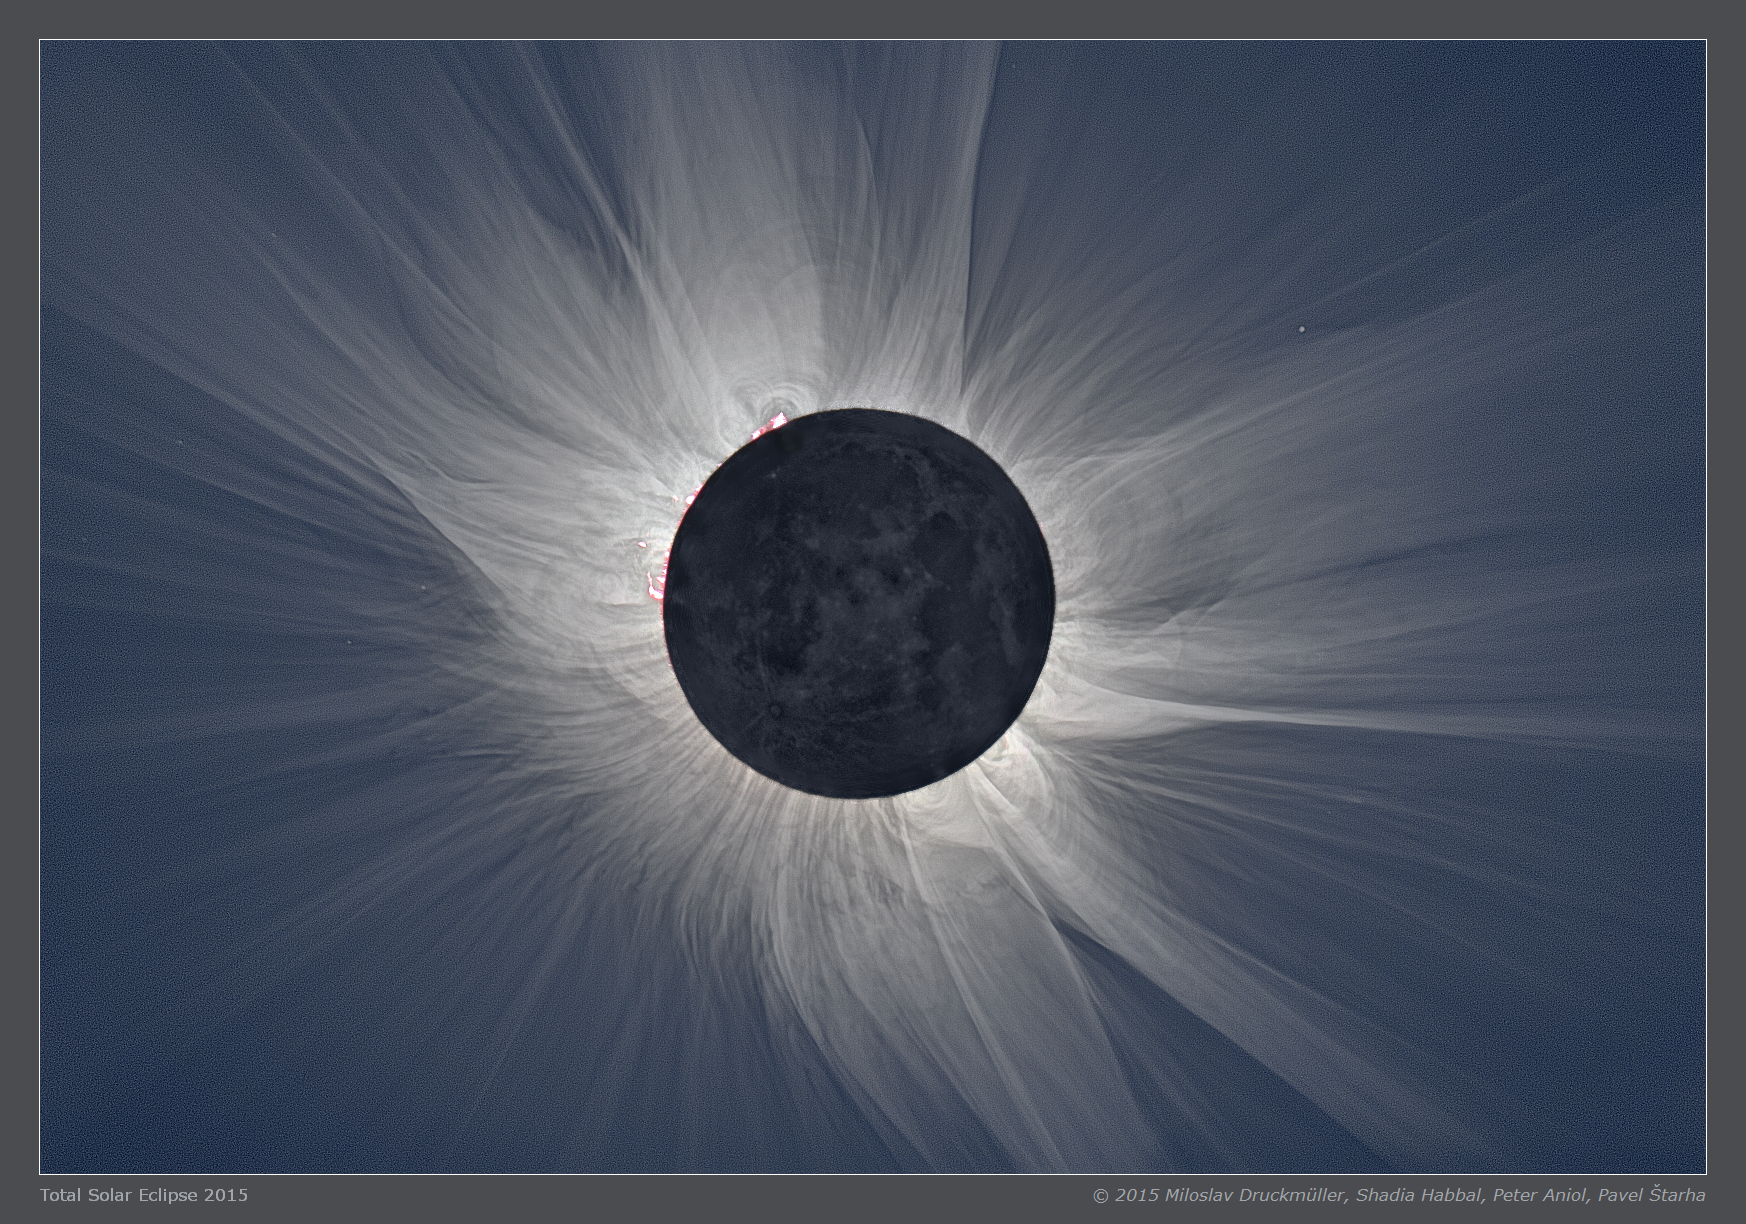
\includegraphics[width=0.7\textwidth]{figures/Tse_2015_Svalbard_800mm_Nikon_D810.png}
	\caption{Total eclipse as seen from Svalbard, Norway on March 20, 2015. Open and closed loops in the highly-structured solar corona are clearly visible. Photo courtesy of Miloslav Druckm\"{u}ller.}
	\label{fig:solar_eclipse}
\end{figure}
%
\par In particular, solar eclipses have captured the attention of artists for centuries. Cosmas Damian Asam, a Bavarian painter and architect active in the early eighteenth century, used images of solar eclipses in many of his works, including several frescoes and an altarpiece. \citet{olson_st._2007} discuss how Asam, a deeply religious artist, was commissioned several times to depict the vision of St. Gregory the Great, a Benedictine monk, as described in his work \textit{Dialogues}. 
%
\par One of these depictions, an altarpiece at a Benedictine monastery in Kladruby, Czech Republic (see Fig. 7 of \citet{olson_st._2007}), shows ``the visionary globe surrounded by a glowing halo of yellow light that more closely resembles the solar corona'' \citep{olson_st._2007}. An additional altarpiece at another monastery in Weltenburg, Germany shows a perhaps even more pronounced depiction of the solar corona during a total solar eclipse. \citet{olson_st._2007} note that, given his detailed depictions, Asam must have observed several solar eclipses as well as the solar corona, with these astronomical events profoundly impacting his depictions of supernatural events in his works. This is but one example of how solar eclipses and their consequential insight into the highly structured solar atmosphere, have shaped scientific and artistic discourse througout history.
%
\hl{maybe here need some info on observing instruments, SDO/AIA, Hinode, Yohkoh, TRACE, IRIS, Hi-C; talk of early observations probably easily transitions into discussion of more modern observations, understanding of the Sun/corona need some sort of wrap-up for this section; maybe also add something here about practical applications/space weather?}
%%
\section{Structure of the Solar Atmosphere}
\label{sec:structure}
\par Though the Sun can be easily seen from Earth, its dynamic and highly structured atmosphere is not observable with the naked eye, with the one exception being brief glimpses of the corona during an eclipse. The interior of the Sun is of course very complex and constitutes a very different regime of physics than that seen in the solar atmosphere. Thus, this work will be primarily limited to the upper solar atmosphere with some discussion of the lower layers.
%
\par The solar atmosphere is often divided up into four separate regions: the photosphere, the chromosphere, the transition region, and the corona. Fig. \ref{fig:cartoon_layers} shows a cartoon of the different layers while Fig. \ref{fig:graph_layers} shows the density and temperature profiles of the atmosphere with each region labeled. The \textit{photosphere} is what we typically refer to as the solar surface, with the actual surface located where the optical depth, $\tau$, is equal to 1. This region also contains the lowest temperature on the Sun, approximately 4400 K, located about 525 km above the surface \citep{carroll_introduction_2007}. The photosphere is where the majority of the visibly (with the naked eye) observable photons originate.
%
\par The temperature minimum defines the top of the photosphere above which lies the \textit{chromosphere}. As can be seen from Fig. \ref{fig:graph_layers}, the density in the chromosphere is many orders of magnitude less than that of the photosphere and the temperature has increased from the minimum up to about $1\times10^4$ K. Though not visible with the naked eye, the chromosphere is highly structured. Structures such as spicules, tall columns of gas that extend high into the solar atmosphere thought to heavily impact the behavior of plasma in the corona \citep{de_pontieu_origins_2011}, originate in the photosphere as well as filaments, essentially spicules observed on-disk and plage, bright regions surrounding sunspots.
%
\begin{figure}[htbp]
	\centering
	\subfigure[]{%
	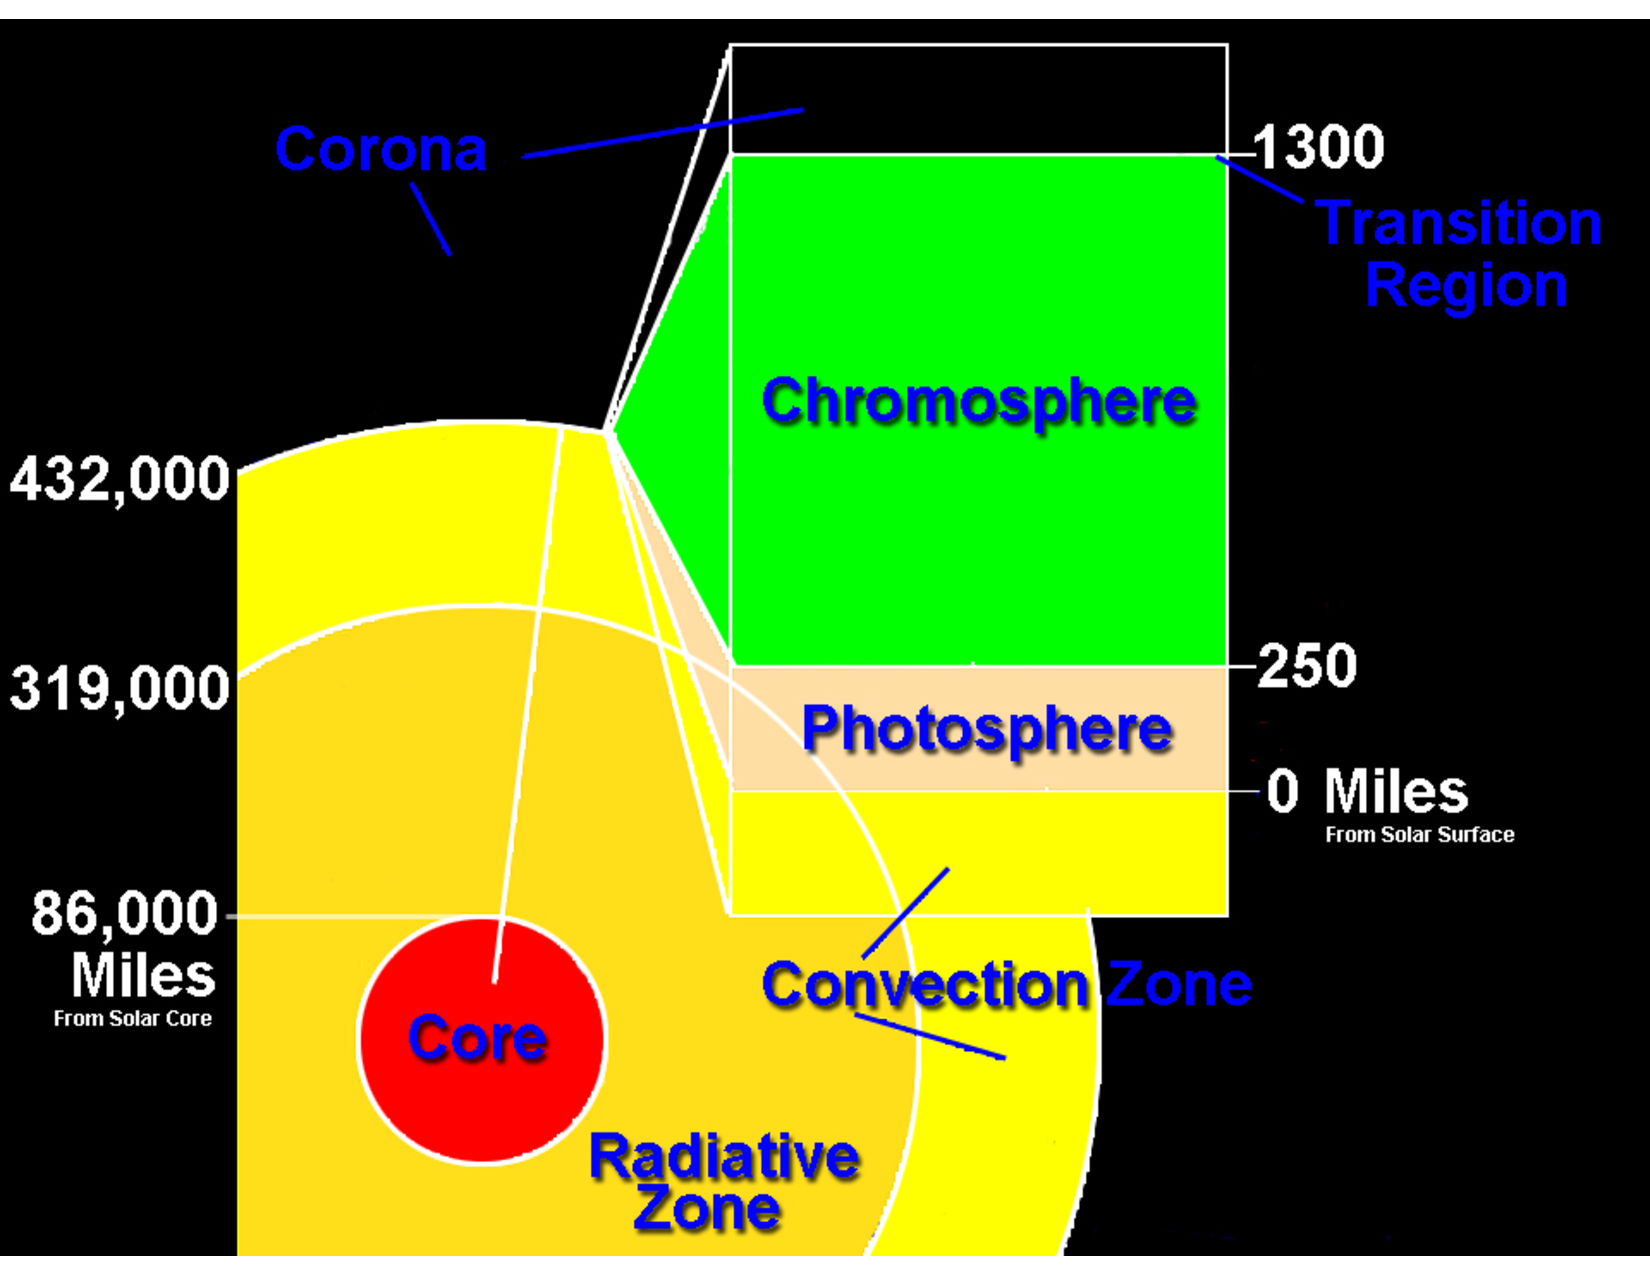
\includegraphics[width=0.45\textwidth]{figures/cartoon_layers.pdf}
	\label{fig:cartoon_layers}}
	\subfigure[]{%
	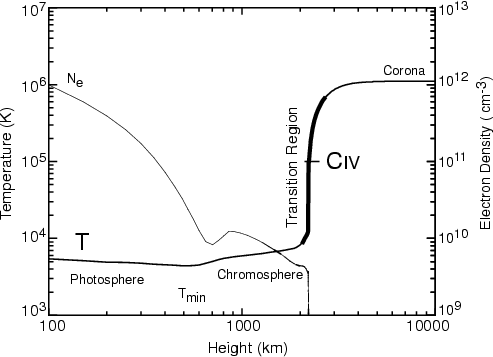
\includegraphics[width=0.45\textwidth]{figures/diagram_layers.png}
	\label{fig:graph_layers}}
	\caption{\textbf{(a)} Schematic showing the layers of the solar atmosphere; the corona is the uppermost layer of the atmosphere. Courtesy of NASA \textbf{(b)} Temperature and density as a function of height above the solar surface; the corona is characterized by low densities and anomalously-high temperatures. Taken from \citet{gary_solar_2007}}
	\label{fig:layers}
\end{figure} 
%
\par Next is the \textit{transition region}, so called because of the steep temperature and density gradients (see Fig. \ref{fig:graph_layers}) that mark the transition between the chromosphere and the corona. The transition region is extremely thin, only a few hundred kilometers as compared to the chromosphere which extends over many thousands of kilometers. However, in this very short change in altitude, the temperature in the solar atmosphere jumps from $\approx1\times10^4$ K to temperatures exceeding $1\times10^5$ K. 
%
\par Finally, the solar \textit{corona}, or ``crown'', is the highly-dynamic uppermost layer of the Sun's atmosphere. Visible with the naked eye only during a total solar eclipse (see Fig. \ref{fig:solar_eclipse}), the corona is highly-structured and diffuse. Here, the temperature continues to increase, with typical coronal temperatures exceeding $1\times10^6$ K. Particularly high temperatures ($\approx1\times10^7$ K) have also been observed in \textit{active regions}, sites of intense magnetic activity associated with sunspots. These active regions can contain plasma as cool as $1\times10^4$ K as well and represent some of the most dynamic portions of the solar corona.
%
\par The work presented here will focus primarily on the plasma dynamics in the corona, in particular, in the cores of active regions where the intense magnetic field drives the motion of the plasma. In the following sections, we will discuss the origin of the solar magnetic field, its topology, how it impacts plasma in the solar corona, and finally how it connects to the anomalously high temperatures seen in the upper solar atmosphere.
%%
\section{The Solar Magnetic Field}
\label{sec:magnetic_field}
\par Because of the high temperatures that characterize both the solar atmosphere and interior, much of the gas that makes up the Sun is ionized; that is, each atom has been stripped of at least one of its electrons. This means that the Sun is filled by a sea of charged particles, or plasma. In the corona where temperatures are often higher than $1\times10^6$ K, even heavy elements such as Mg, Ca, and Fe are stripped of their electrons. Because these particles are charged, their motion is strongly dictated by both the electric and magnetic fields via the Lorentz force law. Thus, to understand the dynamics of the coronal plasma, one must first try to understand the magnetic field that ultimately controls it.
%
\subsection{The Solar Dynamo and Flux Emergence}
\label{subsec:dynamo_flux}
\par The Sun, like the Earth, possesses an intrinsic magnetic field, though its origin and dynamics constitute a largely unsolved problem. Additionally, unlike Earth, the solar magnetic field is highly dynamic and comparatively quite strong (up to 1000 G in sunspots as compared to the $<1$ G field on Earth) \citep{aschwanden_physics_2006}. From the earliest studies of magnetism, it has been known that a conductor moving through a magnetic field produces a current. This current then in turn produces an additional magnetic field. Treating the convection zone (below the photosphere) plasma as the conductor and assuming some preexisting, but small magnetic field leads to what is commonly known as \textit{dynamo theory} \citep{golub_solar_2010}.
%
\begin{figure}[htbp]
	\centering
	\subfigure[]{%
	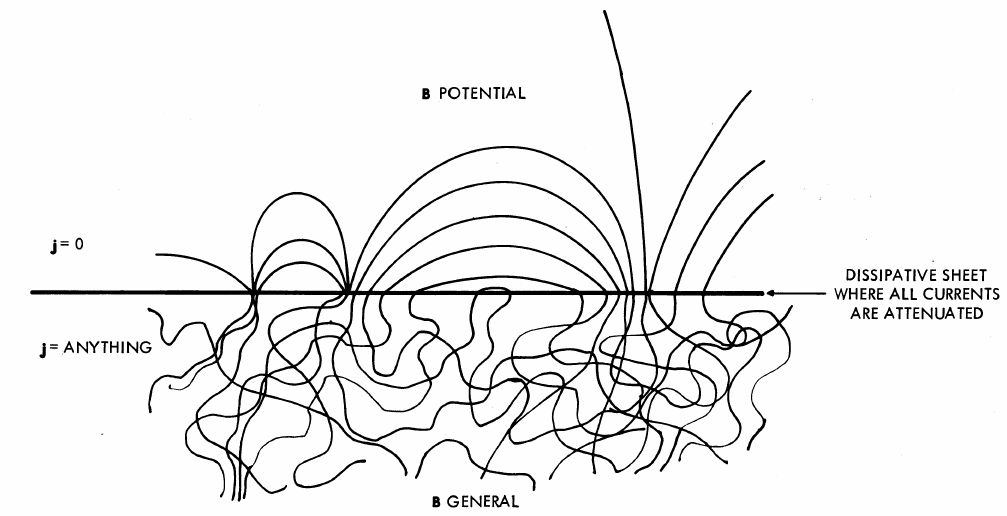
\includegraphics[width=0.60\textwidth]{figures/piddington_cartoon.png}
	\label{fig:cartoon_flux}}
	\subfigure[]{%
	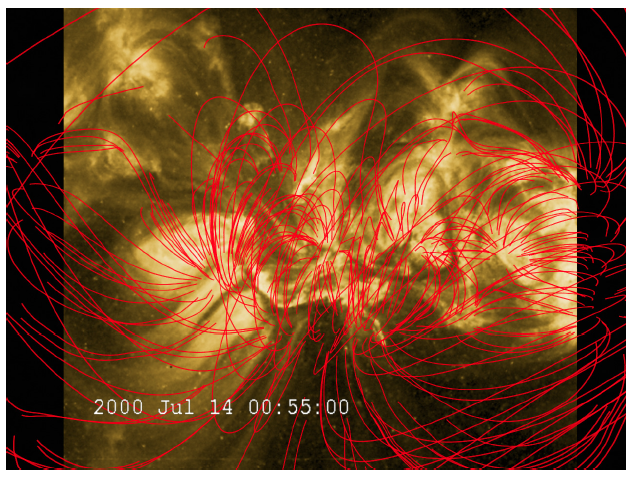
\includegraphics[width=0.35\textwidth]{figures/mag_field_extrapolation.png}
	\label{fig:mag_extrap}}
	\caption{\textbf{(a)} Flux emergence from twisted and tangled field below the photosphere yields loop structures that stretch high into the solar atmosphere. Taken from \citet{gold_magnetic_1964}.\textbf{(b)} The coronal magnetic field topology is extremely complex, making determinations of coronal plasma dynamics difficult. Shown here is a magnetic field extrapolation constructed from an optical magnetogram. An image from the TRACE satellite is superimposed to show the loop structures. Taken from \citet{reale_coronal_2010}.}
	\label{fig:complex_fields}
\end{figure}
%
\par Dynamo theory seeks to show self-consistently how the interaction between the Sun's hot plasma and some small initial field leads to the observed complicated topologies and field strengths. Modeling such a system is no easy task as the interactions between the field and the plasma are highly non-linear, meaning solving the so-called ``dynamo equations'' requires a significant amount of computational effort. But how does this field affect the plasma dynamics of the corona? The solar magnetic field is said to be \textit{frozen in} to the solar plasma; that is, the field moves with the plasma. Since the Sun is not solid, it undergoes \textit{differential rotation}, meaning that different latitudes are spinning at different rates. Since the field follows the motion of the plasma, this causes the normally dipolar (north-south aligned) field to have an east-west component. This amplified and twisted field is then carried up to the photosphere by magnetic buoyancy, an idea first proposed by \citep{parker_formation_1955}, resulting in dipolar loop-like structures poking through the solar atmosphere (see Fig. \ref{fig:cartoon_flux}). This phenomenon, commonly referred to as magnetic flux emergence, is by no means a solved problem and is a continuing topic of research \citep[see][]{cheung_flux_2014}. Finding out how the solar magnetic field is generated and how it makes its way to the upper atmosphere will undoubtedly help to explain much of the observed plasma dynamics in the corona. 
%
\begin{figure}[htbp]
	\centering
	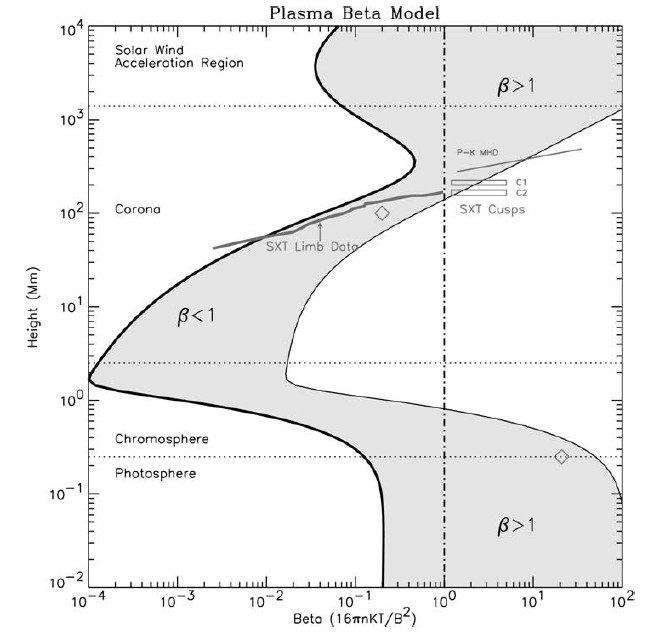
\includegraphics[width=0.6\textwidth]{figures/plasma_beta.png}
	\caption{Evolution of $\beta$ as a function of height in the solar atmosphere. In the chromosphere, the gas pressure dominates ($\beta>1$) while in the corona, the opposition is true, making cross-field motion negligible. Out in the solar wind, the plasma returns to $\beta>1$. Taken from \citet{gary_plasma_2001}.}
	\label{fig:plasma_beta}
\end{figure}
%
\subsection{Magnetic Reconnection}
\label{subsec:magnetic_reconnection}
\par After the magnetic field is forced into the solar atmosphere by the bouyant motion of the convective zone, it remains rooted in the photosphere, whether it is an \textit{open} (flux tube extends radially outward, possibly connecting with the interplanetary magnetic field) or \textit{closed} (both ends attached to the solar surface) field line. Because the field is \textit{line-tied}, or frozen into the photospheric plasma, the turbulent motion of the photosphere deforms and stresses the overlying field, leading to the storage of magnetic energy. This motion can eventually lead to a topological restructuring of the magnetic field as it relaxes from a stressed to an equilibrium state, a process popularly known as \textit{magnetic reconnection}.
%
\begin{figure}[htbp]
	\centering
	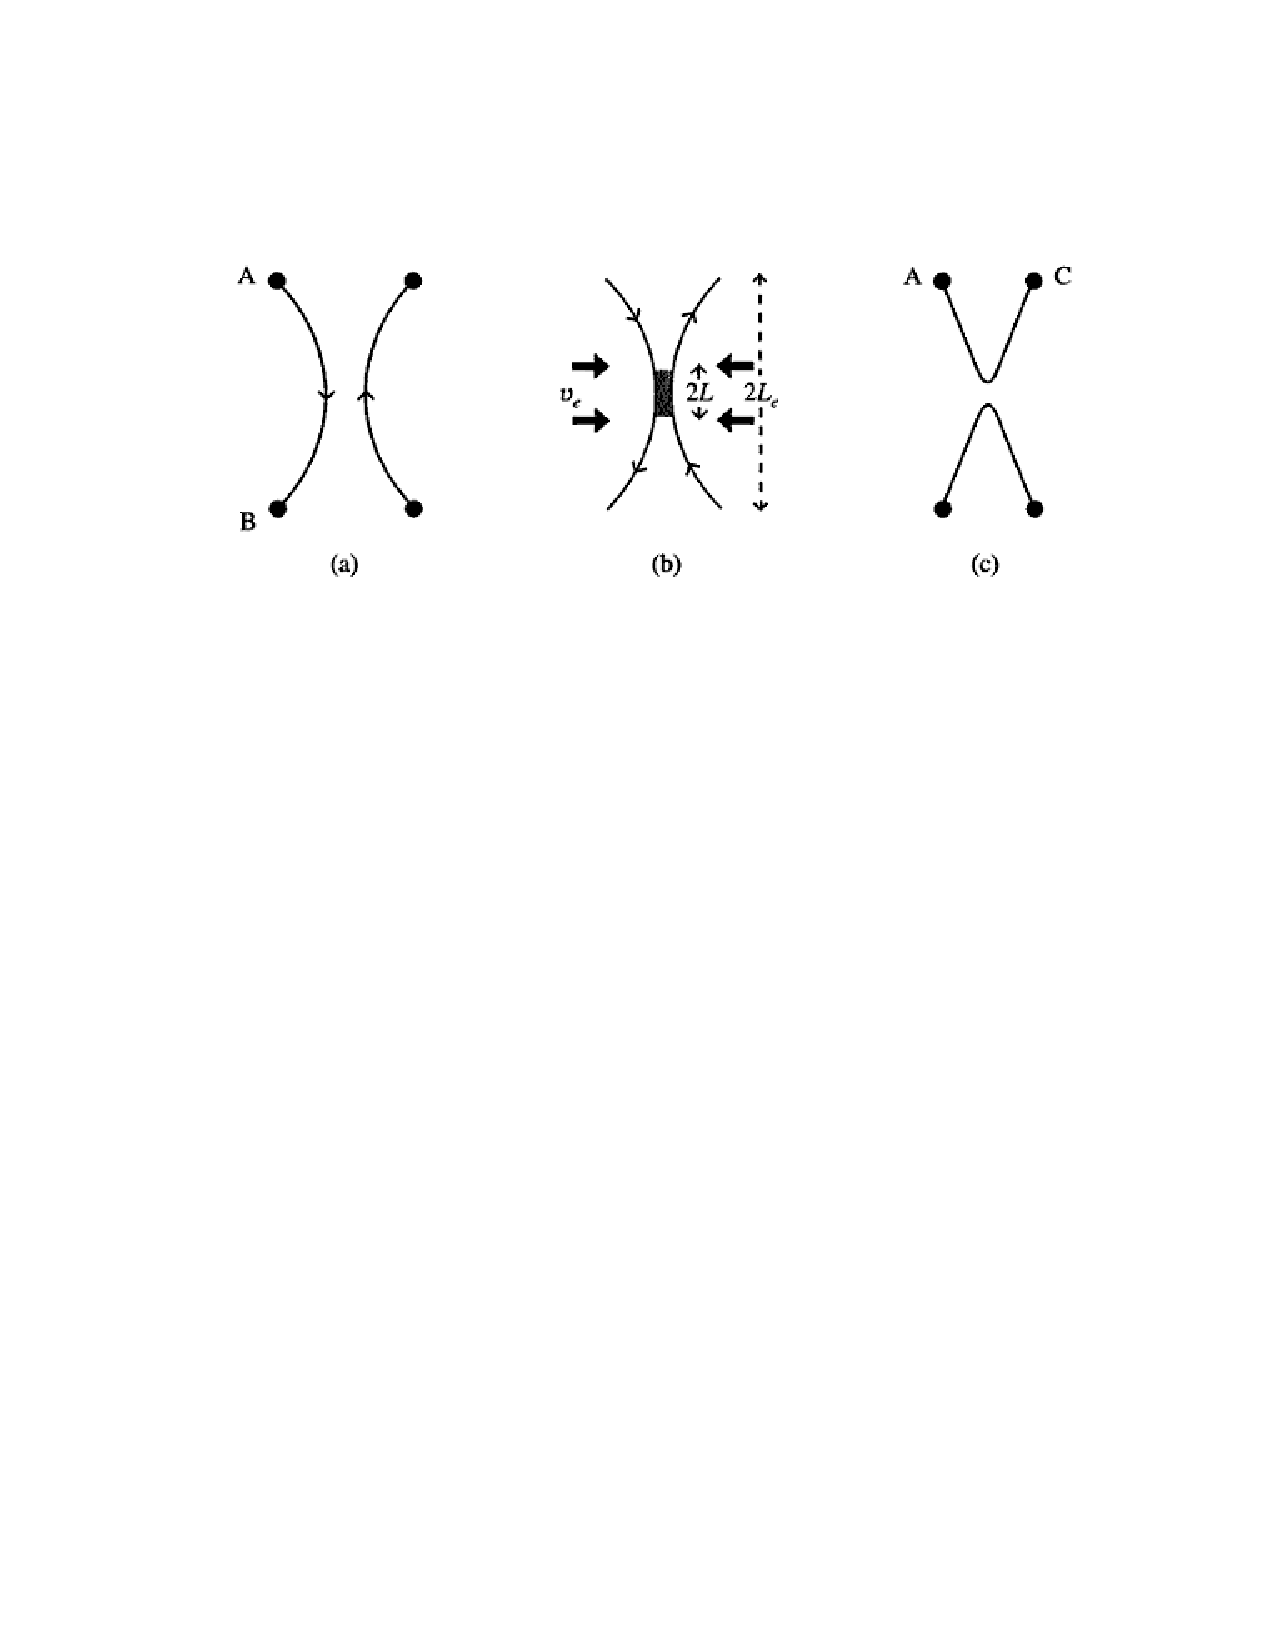
\includegraphics[width=0.6\textwidth]{figures/reconnection_cartoon.pdf}
	\caption{Cartoon showing basics of reconnection process. Image taken from \citet{priest_magnetic_2000}.}
	\label{fig:reconnection}
\end{figure}
%
\par Magnetic reconnection is thought to be a dominant process in a variety of space and astrophysical plasma environments, including Earth's magnetosphere, solar flares, and accretion disks. Additionally, reconnection has also been observed in laboratory settings such as the tokamak and the reversed field pinch \citep{priest_magnetic_2000}. It is also thought to be the primary driver of some coronal heating mechanisms (see \S\ref{subsec:dc_heating}). The basic idea behind reconnection is illustrated in Fig. \ref{fig:reconnection}. When two oppositely-directed field lines are brought together in a conducting fluid (such as a plasma), a tangential discontinuity develops between them with current-carrying plasma squeezed into this area of discontinuity. Because the field lines are frozen into the plasma, a large magnetic gradient develops at the discontinuity in an area called the \textit{diffusion region} (the gray box in Fig. \ref{fig:reconnection}). Because of these large gradients, the resistivity in this region becomes very high, allowing the magnetic field lines to diffuse through the plasma, reconnect, and relax to a topologically different, but more energetically favorable state. As the field lines reconnect and are pushed out of the diffusion region, they accelerate and heat the plasma. Reconnection is thus a non-ideal process as it allows for the conversion of stored magnetic energy to kinetic and thermal energy via dissipation \citep{priest_magnetic_2000}.
%
\par Research into magnetic reconnection has been continually driven by the desire to understand fundamental processes in astrophysical plasmas, primarily those that heat the corona and lead to solar flares. The first complete theory of reconnection was proposed by \citet{sweet_neutral_1958} and \citet{parker_sweets_1957,parker_solar-flare_1963}. In the Sweet-Parker model, as it is popularly known, a diffusion region of length $2L$ and width $2\ell$ is defined between two anti-parallel fields. The field lines are carried into the diffusion region with speed $v_i=\eta/\ell$, where $\eta$ is the magnetic diffusivity. Using Maxwell's equations and the mass and momentum conservation equations from magnetohydrodynamic (MHD) theory, the inflow velocity, or reconnection rate, can be rewritten as $v_i=v_{Ai}/\sqrt{R_{mi}}$, where $v_{Ai}$ is the Alfv\'{e}n speed and $R_{mi}=Lv_{Ai}/\eta$ is the Magnetic Reynolds number \citep{priest_magnetic_2000}. Unfortunately, the Sweet-Parker model predicts a reconnection rate far too slow to properly account for the energy release timescales observed in flare plasmas. In an effort to remedy the slow reconnection in the Sweet-Parker mechanism, \citet{petschek_magnetic_1964} suggested that magnetoacoustic shocks could provide an additional accleration mechanism for the reconnection rate. Additionally, he proposed a smaller diffusion region, further shortening the reconnection timescale. For many years following Petschek's work, it was thought that the problem of fast reconnection was solved. Today, however, thanks in part to increased computing power that makes three-dimensional and kinetic simulations possible, reconnection is now understood to be a far more subtle mechanism than previously thought, with the Petschek and Sweet-Parker models as only special cases \citep{priest_magnetic_2000}.
%
\par It goes without saying that the solar magnetic field is an extremely complex and dynamic system. Fortunately, one can still gain insight into the solar corona without completely solving the problems of the solar dynamo or magnetic reconnection. The corona constitutes what is commonly referred to as a ``low-beta plasma'' such that $\beta=p_{\mathrm{thermal}}/(B^28\pi)$, the ratio between the gas pressure and magnetic pressure, is $\beta<1$ (see Fig. \ref{fig:plasma_beta}). This means that the coronal magnetic field acts as a guide for the plasma, with the flow directed primarily in the field direction with negligible cross-field motion. A useful analogy is that of water flowing through a pipe: the rigid pipe directs the flow of the water, but has no affect on the underlying fluid dynamics. Provided the field is reasonably stable and the relevant fluid equations are parameterized in terms of the field-aligned coordinate, our equations governing the plasma dynamics need not include the field at all!
%
\par \hl{Talk about drawbacks, mention MHD and hydrodynamic and hydrostatic; lead into coronal heating conversation; not sure if this is actually needed here...}
%%
\section{The Coronal Heating Problem}
\label{sec:coronal_heating}
%
\par Thus, far we have not addressed the important question of why the solar corona is so much hotter than the surface. From an intuitive, thermodynamic perspective, we would expect the atmospheric temperature to decrease as we moved away from the surface. However, nearly 70 years of observations have shown this is not the case and these anomalously high temperatures, dubbed the ``coronal heating problem,'' continue to baffle solar physicists today.
%
\par The discovery of the $>1\times10^6$ K corona was made over the course of nearly fifty years through many laborious spectroscopic observations. Spectroscopic measurements during the late-nineteenth and early twentieth centuries of solar eclipses and images obtained from coronagraphs yielded a suprising result: an unknown line at 5303 \ang, dubbed the ``coronal green line'' \citep{golub_solar_2010}. Because the line could not be associated with any known element, the line was identified as a new element, ``coronium''. Later, more detailed examinations of the coronal spectrum revealed several more unidentifiable spectral lines. \citet{grotrian_zur_1939} showed that many of these lines were due to highly ionized states of heavy elements such as iron and calcium. Additionally, \citet{edlen_deutung_1943} identified four additional coronal lines, Fe X, Fe XI, Ca XII, and Ca XIII, providing more evidence for the presence of highly-ionized atoms in the corona and implying temperatures in excess of $1\times10^6$ K. Because of their work in coronal spectroscopy, \citet{grotrian_zur_1939} and \citet{edlen_deutung_1943} are generally credited with the discovery of the million-degree solar corona. However, some \citep[see][]{peter_discovery_2014} have argued that early coronal spectroscopists did not imply a million-degree corona and that it was in fact Nobel laureate Hannes Alfv\'{e}n, in \citet{alfven_solar_1941}, who first proposed a hot corona, even arguing that it was the interaction between the magnetic field and the charged particles in the solar atmosphere that thwarted our usual thermodynamic intuition. 
%
\par While these early spectroscopic observations are now better understood and a multitude of satellite observations have allowed a much clearer picture of the solar atmosphere, the exact mechanism responsible for the million-degree corona remains unknown. This is certainly not for lack of effort; over the last several decades, many different heating mechanisms have been proposed. These are traditionally divided into two-separate categories: \textit{AC}, mechanisms that rely on waves to transfer energy from the lower atmosphere into the corona and \textit{DC}, mechanisms that involve dissipation of energy stored in the stressed magnetic field. In order to be successful, a given mechanism must be able to explain the energy source of the heating, how the energy is converted to heat, how the plasma responds and accurately predict any observables from the resulting plasma emission \citep[see Fig. 1 in][]{klimchuk_solving_2006}. 
%
\subsection{AC Heating}
\label{subsec:ac_heating}
\par The same turbulent sub-photospheric motions that stress the magnetic field can also generate waves capable of propagating into the upper solar atmosphere. The AC- or DC-type heating classification depends on the timescale of the stressing motion: if it is longer than a characteristic crossing time of the coronal structure, it is classified as DC heating. If the timescale is shorter than a crossing time, it is classified as AC heating. A variety of wave modes have been observed in both the open and closed corona, including acoustic waves, Alfv\'{e}n waves, and slow- and fast-mode MHD waves \citep{aschwanden_physics_2006}. However, the simple existence of these waves is not enough to make them a viable candidate for coronal heating; they must be able to propagate into the corona with an adequate amount of energy and then efficiently dissipate this energy in order to heat the coronal plasma. For example, acoustic waves are capable of carrying an adequate amount of energy to heat the corona, but are almost entirely reflected by the steep density gradients in the transition region. Alfv\'{e}n waves may also be capable of carrying enough energy to heat the corona, but specific frequencies are required to avoid reflection at the transition region. These particular modes have also been found to be non-dissipative under coronal conditions, making it hard for these waves to actually heat the corona even if they make it to the upper atmosphere \citep{klimchuk_solving_2006}. Wave modes generated in the corona would of course overcome the problem of crossing the transition region boundary. However, while oscillations in the corona have been observed \citep{de_moortel_longitudinal_2002,de_moortel_longitudinal_2002-1}, the properties of these waves have not been measured precisely enough to say whether or not they are capable of heating the corona \citep{klimchuk_solving_2006}.
%
\subsection{DC Heating}
\label{subsec:dc_heating}
\par As discussed in \S\ref{sec:magnetic_field}, the magnetic field that extends into the corona is rooted in the photosphere. Because of the underlying convection zone, the footpoints of these magnetic loops are subject to a turbulent velocity field and thus undergo a random walk across the surface. The turbulent motion of the footpoints causes the overlying loops to become twisted and braided around each other, leading to a highly stressed magnetic field above the solar surface. \citet{gold_magnetic_1964} first proposed the idea of a twisted field created by photospheric footpoint motions, suggesting that it was the relaxation of the stressed field to its equilibrium (or force-free) state that provided the energy release mechanism needed to power flares. \citet{parker_magnetic_1983,parker_magnetic_1983-1} applied this same concept to the corona and showed analytically that closely-packed magnetic flux tubes are subject to ``dynamical nonequilibrium and reconnection'' and that such a configuration easily leads to braided and twisted field lines with enough free energy to power the corona. Fig. \ref{fig:parker_braids} shows a cartoon of Parker's braided field lines. 
%
\par While \citet{gold_magnetic_1964,parker_magnetic_1983,parker_magnetic_1983-1} included few comparisons to observations (mainly due to the lack of high-resolution instruments of the day), observations from the recently-launched High Resolution Coronal Imager (\textit{Hi-C}) seem to support the idea of magnetic braiding. \citet{cirtain_energy_2013} report two observations, in particular, from the \textit{Hi-C} instrument that show braided magnetic fields, supporting the idea of a DC heating mechanism. \hl{Something here about Hi-C resolution maybe}
%
\begin{figure}[htbp]
	\centering
	\subfigure[]{%
	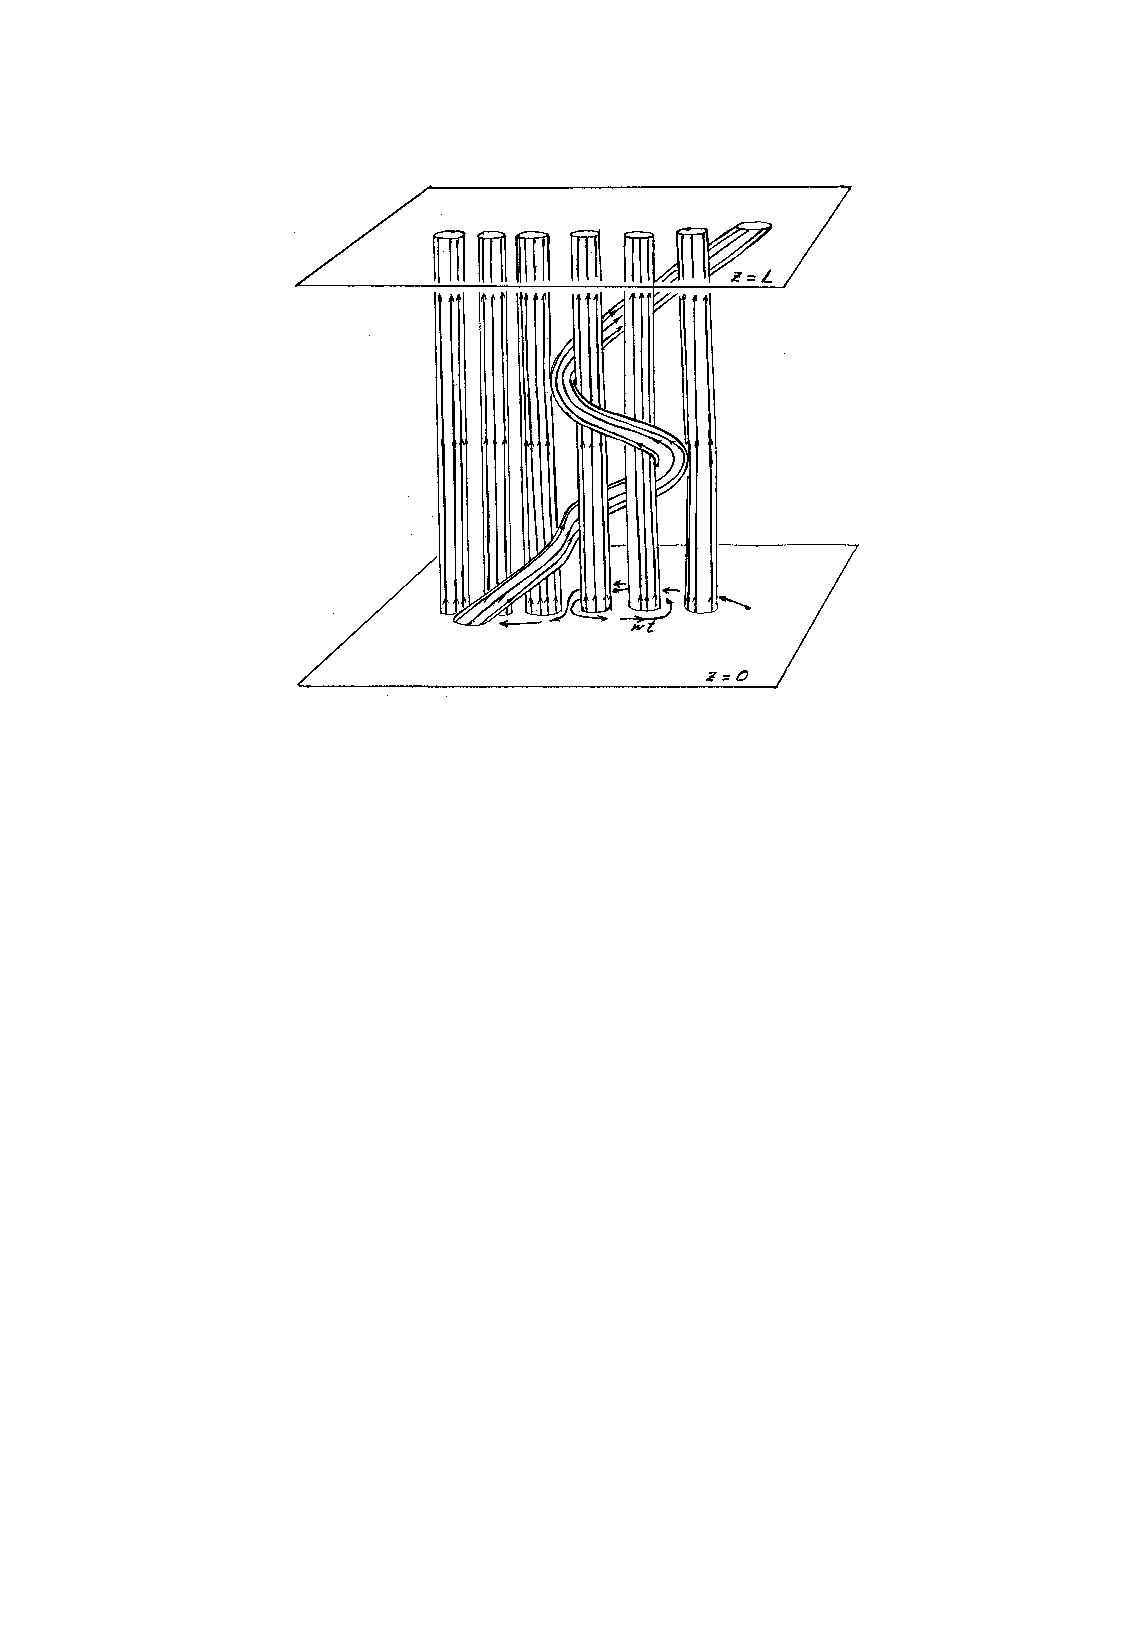
\includegraphics[width=0.4\textwidth]{figures/parker_braids.pdf}
	\label{fig:parker_braids}}
	\subfigure[]{%
	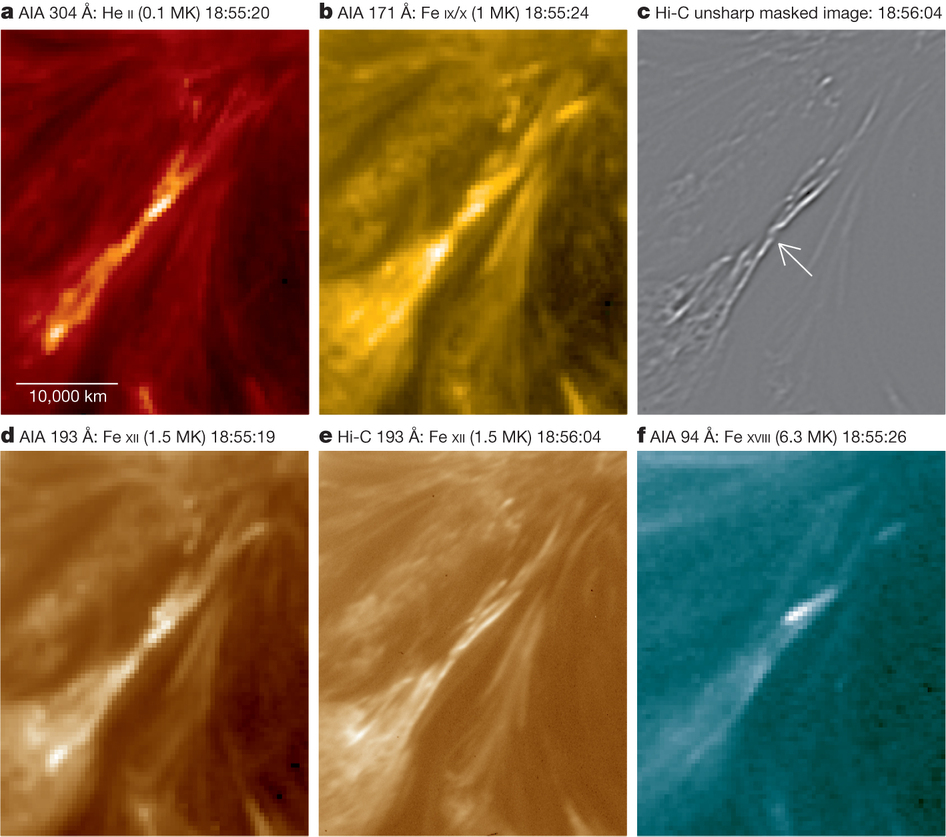
\includegraphics[width=0.55\textwidth]{figures/hi_c_braids.png}}
	\caption{\textbf{(a)} Cartoon showing braided flux tubes rooted, or line-tied, to the solar surface. Braiding allows for the build-up and relaxation of the field, providing an energy release mechanism capable of heating the solar corona. Taken from \citet{parker_magnetic_1983-1}. \textbf{(b)} Image from the \textit{Hi-C} sounding rocket mission showing spatially-resolved braided flux tubes in the solar corona. Image taken from \citet{cirtain_energy_2013}.}
	\label{fig:coronal_braids}
\end{figure}
%
\par This concept of braided and twisted fields illustrates the basic idea behind DC heating: energy is allowed to build up over time, most likely in the braided and twisted magnetic field as stressed by the turbulent footpoint motions, and then released, most likely through reconnection, as the field relaxes to a near-potential state. Parker expanded on his early coronal heating theory with the now-seminal \citep{parker_nanoflares_1988} in which he proposed that the 2-3 MK temperatures and $10^7$ ergs cm$^{-2}$ s$^{-1}$ observed coronal energy input \citep{withbroe_mass_1977} could be explained by many small, impulsive bursts of energy that he called \textit{nanoflares}. These nanoflares are caused by the many tangential discontinuities that arise in the complex coronal magnetic field, leading to magnetic reconnection and the subsequent dissipation of the mechanical energy stored in the field by the random footpoint motions. 
%
\par For the field, $B$, to become twisted and braided, the footpoints of the loop must have some transverse (with respect to the opposite footpoint, see Fig. \ref{fig:parker_braids}) velocity, $v$ and thus a transverse field component, $B_{\perp}$. It can be shown that the work done on the field, $W$, by the footpoint motion is $W\propto vB_{\perp}B$, such that for $v=0.5$ km S$^{-1}$ and $B=10^2$ G, $W\approx10^7$ ergs cm$^{-2}$ s$^{-1}$, the observed value, when $\theta=\arctan{B_{\perp}/B}\approx14^{\circ}$ \citep{parker_nanoflares_1988}. Using appropriate length scales, the energy per nanoflare event can be estimated as $10^{24}$ ergs, or about one-billionth of the energy of a typical flare. Thus, once $\theta=14^{\circ},$ reconnection dissipates the stored energy and the field relaxes to equilibrium until is wound up again by the footpoint motions, resulting in ``bursty'' energy release with the timescale and energy ultimately determined by the underlying velocity field and dissipation mechanism.
%
\par The Parker nanoflare concept has become one of the most favored and contentious coronal heating models \citep{cargill_implications_1994,cargill_nanoflare_2004,klimchuk_solving_2006}. While many theoretical efforts \citep[e.g.][]{bradshaw_diagnosing_2012,reep_diagnosing_2013} have shown the feasability of nanoflares, the idea has long suffered from a lack observational evidence, though recent high-resolution and high-cadence observations \citep{brosius_pervasive_2014,testa_observing_2013,testa_evidence_2014} have provided encouraging results. The term \textit{nanoflare} has now become synonomous with impulsive heating in the energy range $10^{24}-10^{27}$ ergs, with no specific assumption as to what underlying physical mechanism is responsible for this heating. Thus, in this work, the term nanoflare will refer to bursty energy release on a timescale of approximately 100 s or less.  

%
%%
\section{Summary}
\label{sec:summary}
%
The coronal heating problem is one of the most important unsolved problems in astrophysics. Gaining insight into the complex dynamics of the coronal magnetic field and plasma will allow us to better understand our own Sun and, in particular, how it affects our life here on Earth. Additionally, the field of solar physics has broader applications to fundamental astrophysical processes as studying our closest star will give us a better understanding of how stars throughout the universe behave and evolve. This thesis will focus on the study of coronal heating through the use of hydrodynamic models in which the underlying magnetic field is assumed to be static. In particular, this work will analyze how different heating models affect the emission measure and the resulting observables. This approach, commonly referred to as \textit{forward modeling}, allows one to assess the physical validity of a number of free parameters when compared to observations. \S\ref{ch:coronal_loops} will discuss loop structures in the solar corona with an emphasis on recent observational findings and current modeling techniques. \S\ref{ch:emission} will detail the emission measure diagnostics commonly used in coronal loop physics; in particular, how the line intensities are interpreted and how the differential emission measure (DEM) and other observables are inferred from observations. The details of the efficient hydrodynamic model used in this work will be discussed in \S\ref{ch:numerical}, with particular emphasis given to the improvements made upon previous models. Finally, \S\ref{ch:results} and \S\ref{ch:conclusions} will include the results and conclusions of our study, respectively, with comments regarding future work and improvements included in the latter. 